%PART_3_CHAP_1
\myChapter[tudes écologiques et expérimentales]{\'E}{tudes écologiques~~\break et expérimentales}
%WAIT a Review ok
\begin{resumChap}
Ce premier chapitre de la partie évaluation, a pour but de présenter les points se situant en amont de la recherche, c'est à dire: les outils à disposition, les questions éthiques, les protocoles d'évaluation.\par%
Ainsi, nous commencerons par représenter les différents outils d'analyse qui s'offrent à nous dans le contexte de nos évaluations.\par%
Dans un premier temps, nous évoquerons les moyens qualitatifs mis à notre disposition, puis les moyens quantitatifs; ainsi que, les métriques qui peuvent être constituées; et, bien évidemment, les questionnaires \tiret{standardisés} pouvant être utilisés pour rendre compte objectivement de différents éléments subjectifs à l'individu.\par%
Une fois la question de \gui{comment recueillir les données} posée, nous devons aborder les questions éthiques qui y sont liées, et notamment, quel processus de validation a été nécessaire afin de réaliser notre recherche.\par%
Nous présenterons ensuite les deux méthodologies, et protocoles, mis en place ici, à savoir: une étude écologique longitudinale et une série d'expérimentations ponctuelles; chacune ayant leurs avantages et inconvénients.
\end{resumChap}
\section{Outils d'analyse}
  \subsection{Étude de cas}
    \paragraph{Observation}
        Observer le niveau d’engagement n’est pas toujours évident. Chi et Wylie~\citeB{chi2014icap}, montrent comment découper une tâche en différents états d’engagement: 
        \begin{table}[!h]
            \centering
            \begin{tabular}{|p{0.1\linewidth}|p{0.1\linewidth}|p{0.22\linewidth}|p{0.22\linewidth}|p{0.22\linewidth}|}
                \hline
                ~& \textsc{Passif}\break Recevoir & \textsc{Actif}\break Sélectionner & \textsc{Constructif}\break Générer & \textsc{Interactif}\break Collaborer\\\hline\hline
                \textit{Écouter un cours} & Juste écouter & Répéter, apprendre par cœur, prendre des notes verbatim & Reformuler, schématiser, poser des questions & Confronter son schéma avec autrui, fabriquer un schéma ou des notes communes \\\hline
                \textit{Lire un texte} & Juste lire & Lire à haute voix, souligner, surligner, résumer avec des copié-collés & Auto-explication, fabriquer des tableaux, des schémas, résumer avec ses propres mots & Élaborer et fabriquer sur la contribution de chacun. Mettre en discussion les schémas de chacun \\\hline
                \etc & & & & \\\hline
            \end{tabular}
            \caption[États d'engagement dans une tâche, Chi~\citeB{chi2014icap}]{Exemple d'états d'engagement dans une tâche, Chi~\citeB{chi2014icap}}
            \label{fig:chi}
        \end{table}\par%
        En effet, nous voyons dans cet exemple que la distinction entre un élève passif et actif dans le cas d'une tâche d'écoute n'est pas évident. Il est nécessaire de définir certains critères à quantifier.
    \paragraph{Grille d'analyse} 
        Une difficulté majeure est de définir les critères à quantifier. Par exemple, pour déterminer si un élève est engagé, nous pouvons mesurer, le nombre de questions posées ou, à l'inverse, le nombre de fois qu'il fut distrait (\eg regard vers la fenêtre, bavardage, \etc).
        Une seconde difficulté, est le remplissage de la grille. En effet, il est nécessaire d'avoir un ou plusieurs expérimentateurs présents pour effectuer ce relevé \etou opter pour une solution vidéo, permettant un traitement ultérieur, mais imposant des démarches de mise en place encore plus contraignantes~\citeS{sec:adm}.
    \paragraph{Entretiens}
        Concernant les études de cas, un dernier outil largement utilisé est l'entretien. Il peut être de différentes natures, soit libre: l'intervieweur n'oriente pas le discours; soit semi-directif: l'intervieweur oriente le discours vers différents thèmes définis au préalable par les enquêteurs et consignés dans un guide d’entretien. Cette méthode peut donner lieu à une retranscription écrite totale ou partielle des entretiens ou une simple synthèse~\citeS{sec:entretiens}.
  \subsection{Métriques}
    Pour quantifier objectivement le ressenti (subjectif) qu'a l'utilisateur au cours de son interaction avec un système donné, un certain nombre d'outils ont été mis en place. Ces données peuvent être recueillies de différentes façons. 
    De manière objective, par l'acquisition de signaux biologiques caractéristiques durant l'utilisation de la plateforme (\eg \sht{ECG}, \sht{EEG}, \etc), ou encore par des marqueurs concrets mesurables grâce aux fichiers \textit{log} ou vidéo (\eg temps nécessaire pour réaliser une tâche; nombre d'essais/erreurs; nombre de clics, de sourires; temps de fixation du regard; \etc). Tout comme pour les grilles d'analyses comportementales: du choix des variables sélectionnées dépendra l'interprétation. 
    Une autre manière de mesurer ce ressenti est d'utiliser des questionnaires. Plusieurs versions existent suivant ce qui doit être relevé. Parmi ceux-ci, certains ont fait l'objet d'études poussées afin d'assurer leur validité dans leur version standardisée.\nocite{tricot:edutice-00000154}
    %La validité et la reproductibilité des résultats issus de ce type de mesures sont primordiales pour attester et interpréter les données recueillies de façon pertinente et pérenne.~\citeB{likert1932technique}
  \subsection{Questionnaires}\label{sec:survey}
    \begin{table}[!h]
      \centering
      \begin{tabular}{|l|c|c|l|c|}
        \hline
        \textbf{Type} & \textbf{Nom} & \textbf{Année} & \textbf{Auteurs} & \textbf{nb items} \\ \hline\hline
        Utilisabilité & \sht{SUS} & 1996 & Brooke~\citeB{brooke1996sus} & 10\\ \hline
        Connaissance & Castor & 2018 & Dagiene~\citeB{dagiene2008bebras} & Variable\\ \hline
        Motivation & \sht{POPS} & 1991 & Grolnick~\citeB{grolnick1991inner} & 21\\ \hline
        Motivation & \sht{SPP} & 1982 & Harter~\citeB{harter1982perceived} & 30\\ \hline
        \sht{UX} & \sht{ATT} & 2015 & Lallemand~\citeB{lallemand2015creation} & 28 (4*7)\\ \hline
        Motivation & \sht{IMI} & 1989 & McAuley~\citeB{mcauley1989psychometric} & 42 (7*6)\\ \hline
        Acceptabilité & \sht{NARS} & 2006 & Nomura~\citeB{nomura2006measurement} & 14 (6-5-3)\\ \hline
        Motivation & \sht{QAE} & 2005 & Schiano~\citeB{schiano2005developpement} & 12\\ \hline
        Acceptabilité & \sht{EURO382} & 2012 & \sht{UE}~\citeB{eurobarometer2012382} & 16\\ \hline
        Motivation & \sht{EME} & 1989 & Vallerand~\citeB{vallerand1989construction} & 28 (7*4) \\ \hline
      \end{tabular}
      \caption{Listes des questionnaires retenus, Desprez~\cite{RI}}
      \label{tab:list_survey}
  \end{table}
  \paragraph{Recueil des données}
    Dans de nombreux cas, le recours à une version papier d'un questionnaire pour effectuer les passations est indispensable. En effet, il est rare de disposer d'un ordinateur par personne, notamment lorsque les activités proposées incitent à la répartition en groupe~\citeS{sec:peda}. En revanche, ces copies papier doivent ensuite être enregistrées numériquement afin d'effectuer leur traitement. Ainsi, lorsque le nombre de copies devient grand, il est particulièrement intéressant de se tourner vers des techniques d'\sht{OCR} pour réaliser la numérisation.\par%
    Nous avons choisi pour effectuer ce traitement, \sht{amc}~\citeURL{AMC-QCM}. C'est un logiciel permettant de générer (sous linux et mac) un \sht{pdf} ainsi formaté pour permettre sa reconnaissance future. La source de ce document est au format \LaTeX{}~\citeURL{tibo-QCM}, et de nombreuses fonctionnalités sont présentes. L'ensemble des questionnaires retenus~\citeT{tab:list_survey} ont été proposés dans un format \textit{on-line} ou \sht{pdf} via le site \href{https://www.poppy-education.org/evaluation}{poppy-education.org/evaluation}~\citeURL{tibo-QCM-online}. La plateforme retenue pour les formats on-line fut, pour des raisons de sécurité~\citeS{sec:adm}, la plateforme de sondage en ligne Inria~\citeURL{inria-QCM-online} utilisant le logiciel LimeSurvey (sous licence GNU-GPL).
  %EME
    \paragraph{EME}
    L'\bg{EME} est un instrument mesurant la motivation en éducation créé en 1989 par Robert Vallerand. L’\sht{EME} est formé de 7 sous-échelles mesurant trois types de motivation intrinsèque, trois types de motivation extrinsèque et l’amotivation. 28 affirmations sont à évaluer selon une échelle de: 1 — Ne correspond pas du tout — à 7 — Correspond très fortement — aux raisons pour lesquelles l’étudiant se rend dans son établissement scolaire.~\citeA{pdf:EME}
  %IMI
    \paragraph{IMI}\label{q:imi}
    L'\bg{IMI} est un instrument qui a été développé par Edward McAuley en 1989 pour évaluer l’expérience subjective des participants à travers 7 sous-échelles indépendantes. Chacune de ces sous-échelles se compose (en moyenne) de 6 affirmations et mesure différents déterminants de la motivation intrinsèque des individus. Ici, dans sa version intégrale, l’\sht{IMI} totalise 45 affirmations. Chaque affirmation est à évaluer selon une échelle de: 1 — Tout à fait pas d’accord — à 7 — Tout à fait d’accord–~\citeA{pdf:IMI}
  %POPs
    \paragraph{POPS}
    Le \bg{POPS} est un instrument permettant de graduer la perception qu’ont les enfants de l’implication de leurs parents dans leur quotidien. Créé en 1991 par Wendy Grolnick, il a ici été modifié pour évaluer la perception qu’ont les élèves vis-à-vis de leurs parents et de leurs enseignants. Le \sht{POPS} est composé de 21 affirmations à décliner pour chaque référent (parents et enseignants). Ces 42 affirmations sont à évaluer selon une échelle de: 1 — Pas vrai du tout — à 7 — Très vrai —~\citeA{pdf:POPS}
  %SPP
    \paragraph{SPP}
    Le \bg{SPP} est un instrument créé en 1982 par Susan Harter pour graduer la perception qu’ont les individus d’eux mêmes. Le \sht{SPP} est composé de 30 blocs présentant (pour chacun des blocs) deux profils différents. L’individu est invité à sélectionner le profil le plus proche du sien, puis à le graduer entre — Me ressemble un peu — ou — Me ressemble beaucoup — Plusieurs thèmes sont abordés, comme les compétences perçues, le lien social, l’apparence, \etc. Ce format a pour avantage de décentrer l'individu de lui-même afin d'obtenir une réponse plus objective concernant son ressenti personnel.~\citeA{pdf:SPP}
  %QAE
    \paragraph{QAE}
    Le \bg{QAE} est un instrument créé en 2005 par Schiano-Lomoriello pour déterminer le type de stratégie motivationnelle (approche / évitement dans un but de performance ou de maîtrise) mis en place par l’individu dans l’exécution d’une tâche spécifique~\citeS{sec:accomplissement}. Le \sht{QAE} est composé de 12 affirmations à évaluer selon une échelle de: 1 — Pas vrai du tout — à 7 — Très vrai —~\citeA{pdf:QAE}
  %SUS
    \paragraph{SUS}\label{q:sus}
    \bg{SUS} est un instrument utilisable avec une grande variété de produits et services (matériels, logiciels, appareils mobiles, sites Web, applications, \etc), ici, le kit robotique Poppy ErgoJr. Ce questionnaire se compose de 10 affirmations à évaluer selon une échelle de: 1 — tout à fait pas d’accord — à 7 — tout à fait d’accord —. Créé à l’origine par John Brooke en 1986, une rétrospective parue en 2013~\citeB{brooke2013sus} a montré que ce questionnaire est un outil fiable et rapide et permet de graduer l'utilisabilité~\citeURL{ISO}~\citeS{sec:utilisabilite} et nous apprend que le score moyen obtenu par des dispositifs au SUS est de $68/100$.~\citeA{pdf:SUS}
  %AttrakDiff
    \paragraph{AttrakDiff}\label{q:att}
    L'\bg{ATT}~\citeA{pdf:ATT} est un instrument \tiret{possédant une validation en Français~\citeB{lallemand2015creation}} d’évaluation de l’\sht{UX}. Il a été développé par Hassenzahl, Burmester, \& Koller en 2003~\citeB{hassenzahl2003attrakdiff}. Il est actuellement exploité par la société allemande User Interface Design GmbH, qui propose la passation en ligne gratuitement (en allemand et en anglais) sur son site. La version française de l’\sht{ATT} a été réalisée et validée par Lallemand en 2015. Il se compose de 28 paires d’antonymes. Chaque paire représente des contrastes. %Les 7 échelons entre les deux extrémités vous permettent de décrire l’intensité de la qualité choisie. 
    Les résultats nous renseignent sur les qualités pragmatiques et hédoniques de la plateforme, ainsi que sur son attractivité globale répartie suivant 4 échelles:
    \begin{enumerate}\myItemStyle
    \begin{multicols}{2}
        \item     Qualité Pragmatique
        \item     Qualité Hédonique~-~Stimulation
        \item     Qualité Hédonique~-~Identité
        \item     Attractivité globale
    \end{multicols}
    \end{enumerate}\par%
    La première estime le niveau de difficulté perçu par l'utilisateur.
    La deuxième estime si le dispositif offre une expérience stimulante et novatrice pour l'utilisateur.
    La troisième estime l'intégration sociale perçue avec l'utilisation du dispositif.
    La quatrième estime les mêmes aspects mais d'un point de vue plus global.
  %Euro382
    \paragraph{EURO382}\label{q:euro}
    L'\bg{EURO382} fait partie d’une série d’enquêtes d’opinion, appelée Eurobaromètre, menées au nom de la Commission européenne depuis 1973. Ces enquêtes portent sur un large éventail de questions d’actualité concernant l’Union européenne dans tous ses États membres. L’enquête numéro 382 porte sur l’acceptabilité des robots à travers 16~éléments répartis en 9~questions avec différentes modalités de réponse~\citeA{pdf:EURO382}. Lors de sa première diffusion en 2012 plus de 1000 personnes de chaque pays de l’union européenne ont passé l'\sht{EURO382}. Les résultats de cette étude sont disponibles sur le site européen~\citeURL{euro-data}. Aucune validation statistique n'a été effectuée sur ce questionnaire, ainsi, aucun regroupement de questions n'est possible pour créer des sous-échelles d'analyse. Il est donc nécessaire d'interpréter chacune des questions indépendamment.\par%
    L'\sht{EURO382} se compose donc de 16~éléments répartis en 9~\bg{ques}. La 1\iere de ces \sht{ques} - \textit{Veuillez me dire si vous êtes très intéressé(e), moyennement intéressé(e) ou pas du tout intéressé(e) par les découvertes scientifiques et les évolutions technologiques} - permet d'avoir une première idée de la population étudiée et de son attrait pour le thème ici exposé.
    La 2\ieme~\sht{ques} propose 2~images de robots (\textit{fig.}~\ref{fig:QI2-1}~et~\ref{fig:QI2-2}) et demande d'évaluer - \textit{dans quelle mesure elles correspondent à l’idée qu['ils se font] des robots} - suivant 5 items: \textit{très bien, plutôt bien, plutôt mal, très mal,} et \sht{NSP}.
    La 3\ieme~\sht{ques} cherche à savoir le degré de proximité déjà existant entre le répondant et les robots: à la \sht{ques} - \textit{Avez-vous déjà utilisé [\dots] un robot de ce type [\dots]} - le répondant avait 5 possibilités (et plusieurs réponses possibles): \textit{oui à la maison, oui au travail, oui ailleurs, non, \sht{NSP}}.
    La 4\ieme cherche à déterminer quelle perception pense avoir le répondant sur les robots soit \textit{très ou plutôt positive}, soit \textit{plutôt ou très négative}.
    Les \sht{ques}5 et 8 se composent respectivement de 5 et 4 sous-questions à évaluer respectivement de, \textit{tout à fait d'accord} à \textit{pas du tout d'accord} (sur une échelle de 5 + \sht{NSP}); et de, \textit{tout à fait à l'aise} à \textit{tout à fait mal à l'aise} (sur une échelle de 10 + \sht{NSP}). 
    Ces sous-questions présentent des situations de vie (\ie \textit{Se faire opérer par un robot}, \textit{Faire promener son chien par un robot}) ou des affirmations (\textit{aff.}) telles que: \textit{Les robots volent les emplois des gens}; \textit{Les robots sont une bonne chose pour la société parce qu'ils aident les gens}.
    La robotique et ses applications étant largement transdisciplinaires, les \sht{ques}6 et 7 permettent au répondant d'indiquer dans quels domaines il est nécessaire d'y introduire de la robotique et au contraire dans quels domaines il ne le faudrait surtout pas.
    Enfin la \sht{ques}9 propose aux répondants d'estimer - \textit{Selon [eux] en Europe quand les robots qui remplissent des tâches ménagères deviendront-ils une chose courante} - dans \textit{5, 10, 20ans}, dans \textit{plus de 20ans, jamais, c'est déjà une chose courante} ou \sht{NSP}.
  %NARS
    \paragraph{NARS}\label{q:nars}
    Le \bg{NARS} est un instrument développé en 2004 par l’équipe de T. Nomura~\citeB{nomura2006measurement}.
    Il a pour objectif d’évaluer la perception émotionnelle des robots par les hommes. Il est divisé en 3 catégories d’items: \Li les interactions avec des robots; \ii leur influence sociale; et \iii l’aspect émotionnel des interactions.%Pour les besoins de notre expérience nous avons simplement traduit ce questionnaire de l’anglais vers le français. PAS de trad officiel
    Le \sht{NARS} compte 14 items, 11 négatifs \eg \gui{J’ai peur que les robots aient une mauvaise influence sur les enfants} et 3 positifs \eg: \gui{Je me sentirai à l’aise de parler avec un robot},
    Un score global est calculé en effectuant la somme des items négatifs avec l’opposé de chaque item positif~\citeA{pdf:nars}.
  %Castor
    \paragraph{Concours Castor}
        Le concours Castor~\citeURL{castor} vise à faire découvrir aux jeunes l'informatique et les sciences du numérique. Le concours est organisé tous les ans, au mois de novembre. Il se déroule sous la supervision d'un enseignant, en salle informatique. Le concours dure 45 minutes et comporte environ 12 questions interactives, chacune déclinée en 3 versions de difficulté croissante. Il est gratuit et ne requiert aucune connaissance préalable en informatique. Le concours est ouvert du CM1 à la terminale, et s'adapte au niveau des élèves.
        Le Castor Informatique~\citeB{dagiene2008bebras} a été créé en Lituanie en 2004, et est organisé dans 50 pays, dont la France depuis 2011. Chaque pays organise le concours indépendamment à la même période, en suivant des règles communes. Les pays se réunissent chaque année pour préparer un ensemble de questions, parmi lesquelles chacun effectue sa propre sélection de sujets. Plus de 2 millions d'élèves ont participé à diverses éditions du concours Castor 2017 dans le monde. L'édition Française est organisée par l'association France-ioi, Inria et l'ENS Paris-Saclay, grâce à la contribution de nombreuses personnes.
        De plus, il est possible d'utiliser ces exercices hors concours. Les questions peuvent être individualisées ou même modifiées, le code étant disponible sur GitHub~\citeURL{castor-source}. De plus, de nombreux log peuvent être recueillis par ce biais \eg nombre d'essais, de switching entre les questions, \etc.
  %Autres
    %\paragraph{Autres}
\section{Questions éthiques}\label{sec:adm}
  \subsection{Collaboration et consentement}
    Notre contexte particulier \tiret{la pratique d'activités robotiques avec des élèves mineurs dans leurs établissements scolaires, sur le temps scolaire} a imposé de mettre en place un certain nombre de procédures. 
    Tout d'abord, nous avons dû nous mettre en relation avec le rectorat afin d'accéder à un premier set d'enseignants volontaires pour découvrir le projet. Après leur accord oral, il a fallu, avec l'aide du service juridique Inria, mettre en place un contrat de collaboration entre les établissements scolaires et Inria~\citeA{pdf:contrat}. En effet, il vient préciser les engagements pris entre les deux parties \eg mise à disposition du matériel, la durée de l'engagement, les risques et avantages éventuels, \etc. De plus, il précise également la nature de la recherche, son objectif et les moyens mis en place pour sécuriser les données. À cela s'ajoute le consentement éclairé~\citeA{pdf:consentement} rempli, dans un premier temps par, les enseignants. Puis, les enseignants, en tant que référents de cette recherche auprès de leurs établissements, ont recueilli ce même consentement de la part des tuteurs légaux de leurs élèves mineurs, co-signé par les élèves eux-mêmes.
    Cette disposition spécifique où l'enseignant possède un double statut: sujet de la recherche et membre de l'équipe de recherche, était imposée par le nombre d'élèves potentiellement concernés par la recherche: allant de 15 à 60 élèves (d'une demi-classe à 2 classes complètes) par établissement (une 10\up{zen}) soit théoriquement entre 150 et 600 élèves. Ainsi, les enseignants ont reçu un certain nombre d'indications permettant d'expliciter la recherche aux parents. De plus, une page spécifique du site Poppy Éducation~\citeURL{tibo-QCM-online} a été créée pour \Li stocker les documents nécessaires à la recherche \eg consentement, questionnaires, \etc, et \ii fournir des informations complémentaires \eg protocole de passation, objectifs des questionnaires \etc. Sur cette même page étaient également disponibles les contacts des chercheurs référents à Inria, information aussi accessible à de multiple endroits: consentement éclairé, questionnaires, fiche d'information. Pourtant, aucun parent et / ou élève n'a jamais effectué la démarche de nous contacter directement.
  \subsection{Données personnelles et anonymat}\label{sec:data}
    La collecte des données est un enjeu crucial aujourd'hui, notamment pour celles relevant d'un caractère personnel. Ainsi, ces données doivent être, d'une part anonymisées ou plutôt pseudo-anonymisées. En effet, l'anonymisation totale des données est rarement possible, elle dépend \gui{des moyens susceptibles d’être raisonnablement mis en œuvre, soit par le responsable technique, soit par une autre personne} pour lever cet anonymat (\eg par croisement de données, regroupement, \etc). C'est donc vers une pseudonymisation qu'il faut s'orienter, elle est définie comme suit:
    \citeAtion{pseudonymisation}
    D'autre part ces données doivent être stockées, traitées et surtout sécurisées. Comme est dit dans le formulaire de consentement éclairé~\citeA{pdf:consentement}, signé par l'ensemble des participants (enseignants, tuteurs légaux des élèves mineurs et élèves), les mesures suivantes ont été appliquées pour assurer la confidentialité des renseignements fournis par les participants:
    \begin{itemize}\myItemStyle
        \item Les noms des participants ne paraîtront dans aucun rapport
        \item Les divers documents de la recherche seront codifiés et seul le chercheur aura accès à  la liste des noms et des codes
        \item Les résultats individuels des participants ne seront jamais communiqués 
        \item Les matériaux de la recherche, incluant les données et les enregistrements, seront conservés (ex:  lieu, matériel sous clé ou données sur ordinateur protégées par un mot de passe [chiffrement par AES-256\footnote{Advanced Encryption Standard ou AES: algorithme de chiffrement symétrique, Joan Daemen et Vincent Rijmen, Première publication: 2000}] ). Ils seront détruits 10 ans après la fin de la recherche 
        \item La recherche fera l'objet de publications dans des revues scientifiques, et aucun participant ne pourra y être identifié ou reconnu directement ou indirectement 
        \item Un court résumé des résultats de la recherche sera expédié aux participants qui en feront la demande en indiquant l’adresse où ils aimeraient recevoir le document, juste après l’espace prévu pour leur signature 
        \item Dans un souci de protection, la liste des noms et des contacts des participants sera conservée pendant 1~an puis détruite
    \end{itemize}\par%
    De plus, comme toujours dans ce contexte et conformément à la loi Informatique et Libertés n°78-17 du 6 janvier 1978, les participants disposent d’un droit d’accès et de rectification à leurs données nominatives. Et, s'ils décident de mettre fin à sa participation, les renseignements personnels le concernant seront alors détruits.
    Cependant, seuls les enseignants possèdent des données nominatives, en l'occurence, le fichier croisant \cro{nom} et \cro{identifiant unique}. Car, en effet, les questionnaires, bien qu'anonymes, devaient pouvoir être identifiables pour permettre l'appareillage des résultats des différentes passations des individus tout au long de l'année. D'où l'emploi du terme: pseudonymisation.
  \subsection{Outils de recueil}
    Comme mentionné précédemment~\citeS{sec:survey}, nous avons sélectionné deux formats de recueils pour effectuer les passations. 
    Le 1\ier est un format en ligne, utilisant le framework LimeSurvey~\citeURL{LimeSurvey} (sous licence GNU-GPL) et hébergé sur les serveurs propres de Inria~\citeURL{inria-QCM-online}. Ceci, garantissant la sécurisation et le traçage des données lors du recueil. Ensuite, ces données (non-nominatives) sont exportées sous forme de tableur et chiffrées immédiatement via la suite logiciel LibreOffice qui permet une sécurisation des fichiers par mot de passe avec un chiffrement AES-256. L'architecture et la longueur de toutes les tailles de clés de l'algorithme AES (128, 192 et 256) sont considérées par la NSA\footnote{National Security Agency, un organisme gouvernemental du département de la Défense des États-Unis} en Juin 2013~\citeURL{AES} comme suffisantes pour protéger des documents classifiés jusqu'au niveau \gui{SECRET}. Le niveau \gui{TOP SECRET} nécessite des clés de 192 ou 256 bits. \par%
    Ce même type de chiffrement a été effectué sur les données exportées par le \bg{amc}, notre 2\nd format. C'est un format de passation papier qui possède un fichier source au format \LaTeX{}~\citeURL{tibo-QCM} permettant de générer un fichier \sht{pdf} et un fichier de description: des balises visuelles sur le \sht{pdf} permettent de localiser \tiret{par une technique d'\sht{OCR}}, puis d'identifier \tiret{grâce au fichier de description} les réponses aux différentes questions et de les compiler directement sous forme de tableur.
    Le choix de l'un ou l'autre format était à la charge du reférent de chaque passation, en fonction des contraintes contextuelles. Les deux formats étaient accessibles en ligne via une page dédiée sur le site poppy-education.org~\citeURL{tibo-QCM-online} soit vers un lien de redirection vers la plateforme de sondage Inria, soit via un lien de téléchargement de la version \sht{pdf}.
  \subsection{Validation}
    L'ensemble de ces procédures a dû être soumis à approbation: d'une part, en effectuant une déclaration à la \sbg{CNIL}, comme il convient de réaliser lorsqu'un individu ou un organisme détient une base de données sur une population; et d'autre part, comme il convient dans le cadre d'expérimentation avec des sujets humains, en effectuant la saisine d'un comité d'éthique. Depuis 2011, Inria dispose de son propre comité: le \sbg{COERLE}, et c'est à lui que nous avons fait une \cro{Demande d’Autorisation pour une Recherche impliquant des Sujets Humains}~\citeA{pdf:COERLE}. Après presque 1 an de navette, pour compléter et évaluer notre demande, notre dossier fut accepté, validant notre recherche ainsi que les procédures et moyens mis en œuvre pour la réaliser.
\section{Étude longitudinale}
  \subsection{Avantages et inconvénients}
    Nous avons choisi une démarche écologique pour l'évaluation de nos kits robotiques, à la fois d'un point de vue de leur dissémination et du point de vue de leur impact dans le milieu scolaire français. Cette démarche permet notamment d'intégrer/noyer les biais contextuels (nombre d'élèves par classe; accès aux différents équipements/ressources; heure et localisation des séances; relation inter-élèves; relation enseignant-classe; \etc) aux résultats globaux de notre évaluation, mais aussi, elle impose d'avoir une évaluation sur le long terme. L'ambition ici est d'avoir une évaluation au plus proche des retours d'expériences réelles qui seront faits lors du passage à une plus large échelle. Car, au vu de la multitude de situations spécifiques d'enseignements qui existe, notre évaluation doit rester robuste à tant de variabilité.
    Ici, des résultats qualitatifs issus d'observations et des résultats quantitatifs issus de questionnaires standardisés se complètent pour offrir une meilleure analyse.\par%
    Les retours fournis par les expérimentations ont permis de faire une première évaluation du robot, de sa robustesse, de sa facilité d'utilisation \etc, et de définir des améliorations possibles et de proposer des préconisations comme le temps nécessaire pour construire un robot en classe et le nombre d'élèves par robot. Cela a également permis d'analyser les interactions robots-élèves pour améliorer les ressources pédagogiques proposées. Par exemple, nous avons pu observer le type d'interaction en fonction du nombre d'élèves ou de la personnalité des élèves du groupe.
    Les différentes activités et ressources créées par les enseignants ont été mises en avant sur le forum du projet.
    Nous avons fait le choix d’intégrer l’outil en classe de manière libre, en formant les enseignants, en soumettant des idées mais sans rien imposer. Cela nous a permis d'observer et de chercher à comprendre l’appropriation naturelle qu’ils en ont faite. 
    Pour clôturer la première année du projet et mettre en avant les productions des enseignants et des élèves, un colloque \cro{Robotique et Éducation} de deux jours a été organisé par l'équipe où les enseignants et d'autres partenaires ont présenté leurs travaux et animé des stands de démonstration. Un concours vidéo \cro{les RobOscars} a été organisé pour élire la meilleure production vidéo mettant en avant les robots. La remise des prix s'est déroulée durant le colloque.\par%
    Après cette phase de co-conception, et la validation du \sht{COERLE}, il convenait d'évaluer plus spécifiquement les impacts de l'intégration de cette technologie dans ces enseignements. Ainsi, là où durant la première phase, les enseignants étaient totalement libres de développer telle ou telle pratique, la seconde phase préconisait un protocole plus strict imposant un certain nombre de temporalités~\citeF{fig:proto18}.\par%
    Cependant, ce type de protocole a pour inconvénient d'être plus facilement soumis aux aléas contextuels. En effet, la reforme de 2019 pourtant sur le \sht{Bac}~\citeS{sec:ref_2019} a considérable entravé le bon suivi du programme expérimental le rendant caduc et donc inexploitable. 
  \subsection{Établissements partenaires}\label{sec:etablisements}
    L'intégration de technologies en classe est un processus parfois difficile pour lequel il faut respecter un certain nombre de règles afin qu’elle soit réussie. Baron \& al~\citeB{institut2000technologies} supposent que pour qu’il y ait intégration au niveau des élèves, il importe qu’ils acquièrent une culture globale liée aux outils informatiques. Cette culture ne peut s’obtenir qu’au travers d’une utilisation diversifiée de ces outils avec des tuteurs éclairés. Cet article insiste sur l’importance du choix des terrains; en effet, la recherche des établissements doit être menée dans un but comparatiste. Il est important de préciser comment chacun a été sélectionné, pourquoi, et leurs particularités.
    Dans notre cas, c'est dans un premier temps le rectorat qui nous a aiguillés vers une population d'enseignants volontaires, puis le \cro{bouche-à-oreille} et différents appels à projet ont permis de multiplier les établissements. In fine, selon différents classements existants~\citeURL{classement-ecole},  il y avait une bonne diversité dans les établissements partenaires: urbains / péri-urbains / ruraux et implantés dans des quartiers plus moins défavorisés~\citeA{pdf:etablissements}.
    %D’autre part, la méthode d’investigation doit être précisée. Concrètement, dans cette étude, le chercheur est en contact étroit et prolongé avec les membres du groupe qu’il étudie. Il ne participe toutefois pas à l’intégralité des activités. 
    %Enfin, il est important -pour les auteurs- d’interroger les enseignants et de réaliser des entretiens. Cette démarche a pour objectif de retracer l’historique et d’éclairer sur la situation actuelle des établissements mais également de mettre principalement en évidence ce que les enseignants veulent faire, ce avec quoi ils travaillent habituellement, et les notions que les élèves possèdent déjà~\citeS{sec:entretiens}.
    %Les auteurs insistent également sur d’autres aspects, notamment les divers problèmes de financement et l’influence de ce que les élèves ont a disposition comme outils informatiques chez eux (pouvant notamment influencer sur les stéréotypes qu’ils ont).
  \subsection{Le protocole}\label{sec:proto}
    \subsubsection{En théorie}
        Un certain nombre d’articles donnent des recommandations sur la méthode à utiliser et les principes à respecter afin d’évaluer rigoureusement l’utilité d’une technologie en classe. C’est notamment le cas de Coen \& al~\citeB{coen2006construction} qui préconisent de déterminer en amont et en aval la représentation qu’ont les élèves des technologies, mais également de déterminer le degré d'intégration des technologies, ainsi que le niveau de pénétration de cette innovation sur le terrain (autrement dit, chercher à savoir si elles sont bien acceptées).
        Au cours de cet article~\citeB{coen2006construction}, ils précisent que les effets des technologies en classe sont souvent légers et relativement peu contrôlés. Les auteurs informent que cela est souvent dû à la méthodologie, car le contexte est essentiel à prendre en compte (institutions et acteurs) pour connaître le réel impact des technologies mises en place. L’étude du contexte passe par différents facteurs, notamment l’âge, l'expérience et la motivation des enseignants (qui semblent souvent jouer un rôle sur l'intégration des technologies). L’objectif de l’étude de l’intégration d’une technologie est de regarder les vrais apports et ne pas se contenter de croire que tout changement implique un progrès. Pour cela, les auteurs distinguent 4 caractéristiques principales qui évaluent l’intégration de la technologie: les caractéristiques \Li pédagogiques (selon la conduite des activités pédagogiques), \ii technologiques (selon les aptitudes techniques), \iii psychologiques (attitudes face à la technologie) et \iiii sociales (degré de dépendance et de soutien dont l’enseignant bénéficie).\par%
        Durant la phase de conception aucun protocole particulier n'a été mis en place.
        En fin d'année, il était demandé aux élèves et enseignants de compléter le questionnaire \sht{SUS} et \sht{ATT}, ainsi que le questionnaire \sht{EURO382}. Dont les résultats sont donnés en section~\ref{Exp:L_UX}~et~\ref{Exp:L_ACC}. Pour l'année 2018-2019 et fort des observations informelles réalisées l'année précédente, un protocole rigoureux a été développé~\citeF{fig:proto18}.
      \begin{figure}[!h]
        \centering
        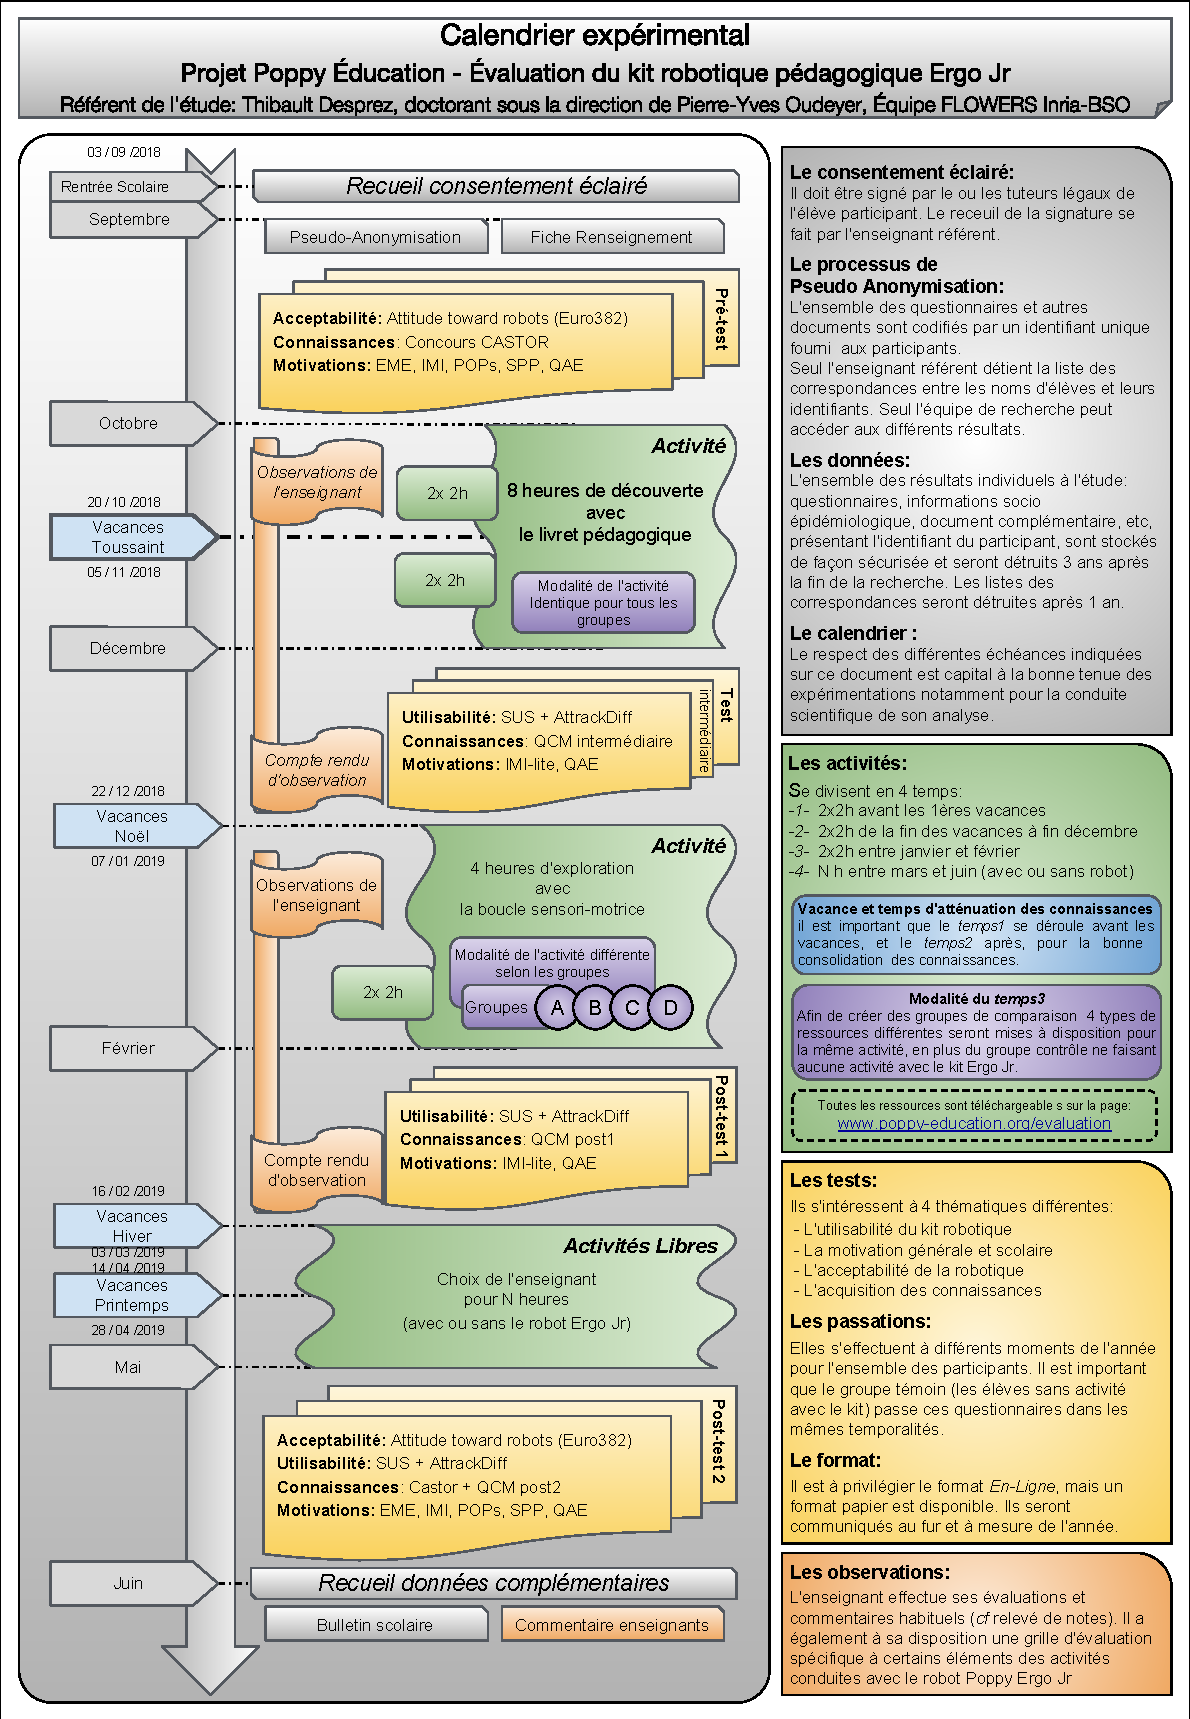
\includegraphics[width=0.9\textwidth]{Annexe/autre/Protocole_2018.pdf}
        \caption{Protocoles d'évaluation expérimentale 2018-2019, Desprez~\cite{RI}}\label{fig:proto18}
      \end{figure}
    \subsubsection{En pratique}
        \paragraph{Les prescriptions}
            Comme nous pouvons le constater sur la plaquette diffusée aux enseignants~\citeF{fig:proto18}, plusieurs temps sont à respecter: en préambule, après la pseudo anonymisation, l'ensemble des questionnaires sélectionnés était à compléter (hormis \sht{SUS} et \sht{ATT}). Courant octobre devait débuter la première série d'activités autour du livret pédagogique, et ce, jusqu'à Décembre, mais en prenant soin de respecter une césure entre les activités, afin de permettre une certaine atténuation des connaissances, garante d'une bonne consolidation de celles-ci pour leur maintien à long terme. Cette 1\iere étape s'est clôturée par une deuxième session de questionnaires, plus courts, ne reprenant que 2 des questionnaires alloués à la motivation, un questionnaire de connaissances et \sht{SUS} et \sht{ATT}. Durant, l'intégralité de cette phase, l'enseignant pouvait constituer une grille d'analyse afin de retranscrire les éléments notoires qu'il remarquait; de même dans la deuxième phase.
            Celle-ci, débutant en janvier, devait se concentrer sur la thématique de la \bg{BSM} \tiret{concept majeur de la robotique} via 4 modalités d'apprentissage et se clôturer par la même série de questionnaires qu'en phase~1 (avec adaptation du \sht{QCM} de connaissances). 
            La troisième phase, était une phase libre où l'enseignant pouvait réaliser n'importe qu'elle activité durant cette période s'étalant jusqu'à la fin de l'année. Juste avant la fin de celle-ci, l'ensemble des questionnaires était complété une ultime fois par les élèves. À noter que chaque enseignant avait à constituer dans son établissement un groupe témoin: complétant les questionnaires (hormis \sht{SUS} et \sht{ATT}), mais ne pratiquant aucune activité avec le kit ErgoJr. 
            Enfin, des données complémentaires devaient être recueillies, notamment pour connaître le set d'activités réalisé pendant la période libre et également pour connaître les taux de réussite globaux des élèves.
        \paragraph{Les réalisations}\label{sec:limit_proto}
            Comme mentionné dans le chapitre 2 de la deuxième partie~\citeS{sec:ref_2019}, la réforme de 2019 concernant le \sht{Bac} 2021 a considérablement impacté la mise en place du protocole écologique. En effet, les enseignants devant préparer la restructuration des filières et surtout la redistribution de certains quotas horaire leur imposant le renouvellement de leurs ressources pédagogiques. Par exemple, le module \sht{NSI} possède un quota horaire supérieur aux filières \sht{ISN} et \sht{ICN} mais rien ne garantit plus la poursuite de l'option sur deux ans. Ainsi, le programme de 1\iere année doit donc pouvoir se suffire en lui-même, là où les activités existantes permettent le report de certaines notions à l'année suivante. De plus, la majorité des enseignants ont également déclaré qu'initialement ils n'avaient pas conscience que le niveau de contrainte des passations expérimentales serait croissant.
            Dés lors, l'intégration de ce protocole dans ce contexte délicat fut un échec, notamment sur le respect des temporalités, et donc aucune donnée fiable n'a pu être extirpée durant cette année. Ainsi, seuls les résultats des questionnaires \sht{SUS}, \sht{ATT} et \sht{EURO382} effectués durant l'année 2017-2018 ont pu donner lieu à une analyse respectivement en section~\ref{Exp:L_UX}~et~\ref{Exp:L_ACC}.
\section{Études ponctuelles}
  \subsection{Avantages et inconvénients}
    La mise en place de protocoles écologiques est particulièrement longue et contraignante. De plus, les résultats ne sont pas toujours exploitables. 
    C'est l'une des raisons pour laquelle nous réalisons en parallèle des expérimentations plus directes. Elles ont l'avantage d'être plus faciles à mettre en place, car moins dépendantes des contextes extérieurs: elles se réalisent sur des sessions courtes et autonomes entres elles, avec notre propre matériel et sous notre contrôle.
    L'objectif de ces études en environnement contrôlé est avant tout de mettre en évidence certains biais contextuels et leur influence possible sur les expérimentations écologiques pour pouvoir les contrôler au mieux. Un autre objectif est d'étudier plus finement des éléments qui, en contexte écologique, seraient totalement noyés sous l'influence d'autres facteurs. Cependant, on peut s'interroger sur la pertinence de tels déterminants ainsi mis en évidence, si, dès lors que l'individu est placé en milieu écologique, leurs effets ne sont plus réellement mesurables.
    Ainsi, mener en parallèle ces deux types d'études permet de les compléter l'une l'autre.
  \subsection{Protocole global}
    Durant ces études ponctuelles, un protocole général a été établi.
    Les sujets se répartissent en groupe de 2 ou 3 (suivant les sessions). Chaque mini-groupe a à disposition, un robot, un ordinateur et les ressources nécessaires à la réalisation de la tâche. La moitié des mini-groupes dispose d'un matériel \cro{à tester} l'autre moitié, représentant le groupe contrôle, dispose des ressources classiques. Suivant les cas, ces groupes sont physiquement séparés. En effet, certains éléments visuels ou comportements pourraient faire apparaître aux sujets qu'il existe 2 groupes, chose pouvant biaiser nos résultats.
    Outre le matériel testé, la distinction majeure entre ces sessions porte sur le lieu de passassion \eg dans les classes, à Inria, durant des ateliers ou workshop, ou encore directement sur internet.
    Les protocoles spécifiques à chaque expérimentation sont décrits dans leurs sections respectives~\citeT{tab:list_survey}.